\subsection{Elektronik} \label{cap:methoden_leiterplatte}
Die Leiterplatte wurde im Open-Source Programm \textit{KiCAD} erstellt. \textit{KiCAD} ist eine Computer-unterstützende Zeichnungssoftware, welches erlaubt Elektronische Geräte zu entwickeln. In der Software wird zuerst das Schema gezeichnet. Ein Schema ist ein Plan, welcher angibt, welche Komponente mit welchem Signal verbunden werden. Wurde dieses Schema gezeichnet, kann das Schema in ein PCB (Printed Circuit Board oder Leiterplatte) umgewandelt werden. Eine Leiterplatte ist eine Platte aus Kupfer und Isolationsmaterial mit kleinen Komponenten bestückt. Auf dieser Platte sind nun die Verbindungen, welche im Schema gezeichnet wurden, realisiert.
\newpara
Nachdem das Schema gezeichnet und umgewandelt wurde, konnte mit einer Skizze, welche die grobe Position der Komponenten angibt, die ungefähre Grösse der Leiterplatte selbst bestimmt werden (Siehe Abbildung \ref{fig:board}).


\begin{figure}[ht]
    \begin{center}
      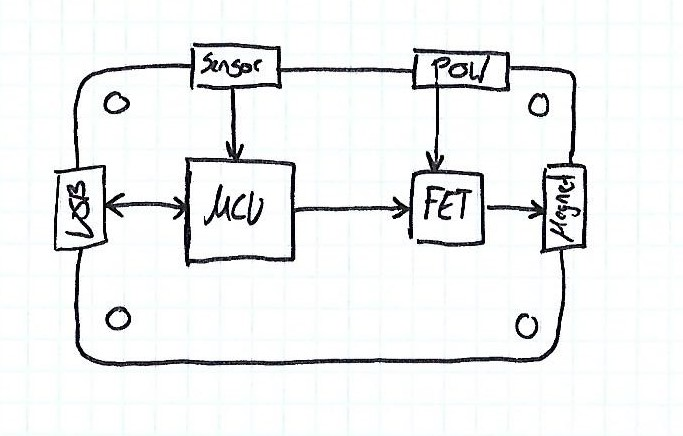
\includegraphics[width=8cm]{assets/images/board}
    \end{center}
    \vspace{-3ex}
    \caption{Skizze des Leiterplattenlayouts}
    \label{fig:board}
  \end{figure}
\newpage


\begin{figure}[ht]
    \begin{center}
      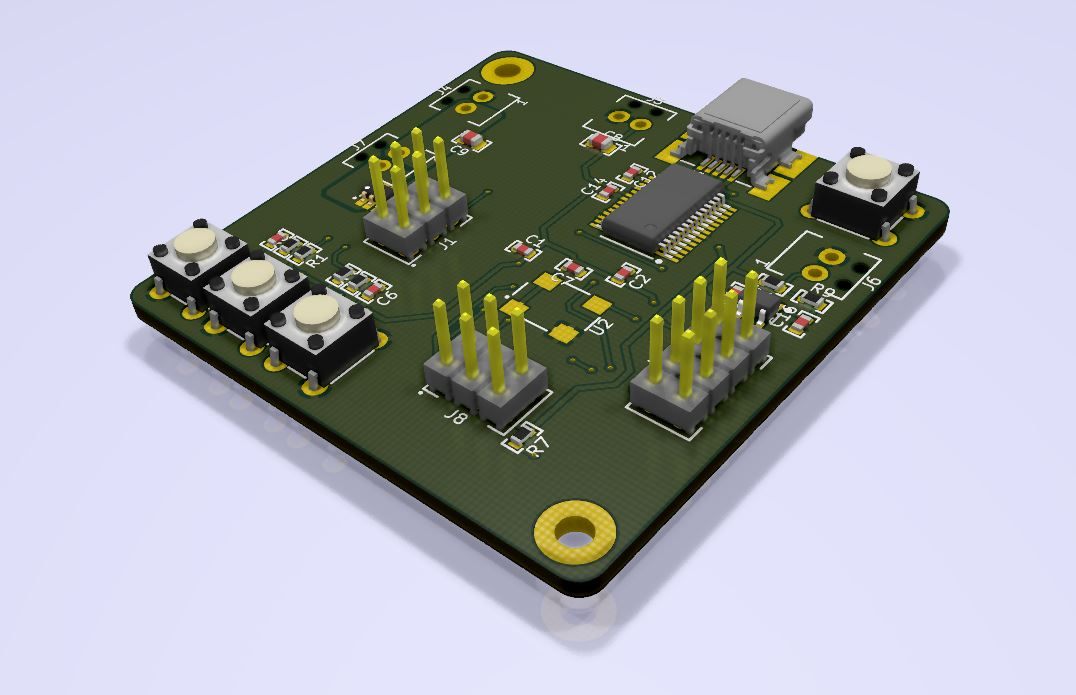
\includegraphics[width=12cm]{assets/images/board_3d}
    \end{center}
    \vspace{-3ex}
    \caption{3D Model der fertigen Leiterplatte}
    \label{fig:3d_board}
  \end{figure}
Nachdem die Leiterplatte fertiggezeichnet wurde (Siehe Abbildung \ref{fig:3d_board}), konnte die Leiterplatte einem Hersteller geschickt werden und die Komponenten konnten bestellt werden.